
%
%  $Description: Author guidelines and sample document in LaTeX 2.09$ 
%
%  $Author: ienne $
%  $Date: 1995/09/15 15:20:59 $
%  $Revision: 1.4 $
%

\documentclass[times, 10pt,twocolumn]{article} 
\usepackage{latex8}
\usepackage{times}

\usepackage{graphicx} %sjr added
\graphicspath{{../presentation/figures/}{../draft/figures/}}
%\documentstyle[times,art10,twocolumn,latex8]{article}

%------------------------------------------------------------------------- 
% take the % away on next line to produce the final camera-ready version 
\pagestyle{empty}

%------------------------------------------------------------------------- 
\begin{document}

\title{Effects of Irregular Topology in Spherical Self-Organizing Maps}

\author{
Charles R. Schmidt\\
School of Geographical Sciences\\Arizona State University\\
Charles.R.Schmidt@asu.edu\and
Sergio J. Rey\\
School of Geographical Sciences\\Arizona State University\\srey@asu.edu
\and
Andr\'e Skupin\\
Department of Geography\\San Diego State University\\
skupin@mail.sdsu.edu
}

\maketitle
\thispagestyle{empty}

\begin{abstract}
We explore the effect of different topologies on properties of self-organizing
maps (SOM). We suggest several diagnostics for measuring
topology-induced errors in SOM and use these in a comparison of four different
topologies. The results $\ldots$
  
\end{abstract}



%------------------------------------------------------------------------- 
\Section{Introduction}

The Self-Organizing Map (SOM) is an unsupervised competitive learning process
developed by Teuvo Kohonen as a technique to analyze and visualize high
dimensional data sets.  The applications of SOM are far reaching;
Kohonen \cite{Kohonen2000} provides a thorough review of the SOM literature including
applications of SOM.  SOM has been used in applications ranging from speech
recognition and image classification to breast cancer detection and gene
expression clustering.  Agarwal
and Skupin \cite{skupin07} outline the growing interest of SOM to
the GISciences, and propose that the relationship between SOM and GIScience
should be bidirectional.  The SOM offers a powerful method for exploring and
visualizing geographic data and GIScience offers a wide array of tools
and methods to enable the exploration of the SOM itself.  The exploration of
spatial relationships has always been of great interest to geographers, and as
Ritter
\cite{ritter99} states, the goal of SOM is ``to translate \emph{data
similarities} into \emph{spatial relationships}'' \cite[p. 1]{ritter99}. 

The SOM is a type of artificial neural network in which neurons are ``organized''
in such a way as to project the high-dimensional relationships of a set of
training data onto a low-dimensional network structure.  The traditional
SOM uses a rectangular or hexagonal network topology \cite{Kohonen2000}.  These topologies 
create a well-known problem in SOM called the boundary or edge effect.  Neurons on
the boundary of the hexagonal and rectangular lattices have fewer neighbors,
which reduces their ability to interact with other neurons during the
self-organizing process.  Using a spherical lattice has been widely suggested as a
solution to the problem \cite{ritter99, boudjemai2003, sangole03,
Nishio:2006fk, wu2006}. The use of the spherical lattice, however, does not
completely overcome the boundary problem, and the choice of which spherical
topology to use for the network can be difficult to make.

A regular network topology is one in which every node on the network has exactly the
same number of adjacent nodes.  Any topology involving an edge is irregular.
Arranging our lattice on the surface of a sphere seems to be an obvious
way to overcome the edge.  However, there exist only five arrangements on the
sphere which are completely regular; these are the five platonic solids \cite{ritter99,
harris2000}.  Any other arrangement of neurons on the surface of the sphere will
result in an irregular topology, as not all neurons will have the same number of
neighbors.

The classic method for minimizing this irregularity is to generate
the spherical lattice by tessellating (subdividing) the sides of the icosahedron
\cite{Nishio:2006fk}.  While this method will always result in a highly
regular spherical topology, the main drawback is that the number of neurons in
the network (the network size), \(N\), grows exponentially as tessellations are
applied. That results in only very coarse control over network size.
 Other methods for arranging neurons on the sphere allow
for unlimited control over network size, but yield topologies with increased
irregularity \cite{harris2000, wu2005, Nishio:2006fk}.  To date the
literature has largely ignored the more irregular methods in favor of the
aforementioned tessellation-based methods.  A topology which yields a more flexible network
size may be desirable.  However, in order to address this issue of network
size, we must first determine the degree to which irregularity effects the
SOM.

\Section{Edge Effects}

An intrinsic problem with SOMs in two dimensions is the so called edge
effect. This is illustrated in  in Figure \ref{f:edge}, which displays a SOM
trained on socioeconomic census data consisting of 32 variables for US states.
The darker a neuron in the figure, the larger is the distance between the
 neuron and mean of the input vectors. The distance between each of the
 original observations (states) and the mean is represented by a graduated
 circle. Taken these two together it is clear that the outlier observations
 are pushed towards the edges of the map, while the observations that are
 closest to the multidimensional center of the data are assigned to central
 neurons on the map.

At the edge of the map, neurons have fewer neighbors which results in any
observations being assigned to them having fewer competitive signals. At the
same time, the edge of the neural lattice represents a true visual boundary
which affects its ability to represent data similarities as spatial
relationships.

\begin{figure}
  \begin{center}
\caption{Edge effects in SOM}\label{f:edge}
  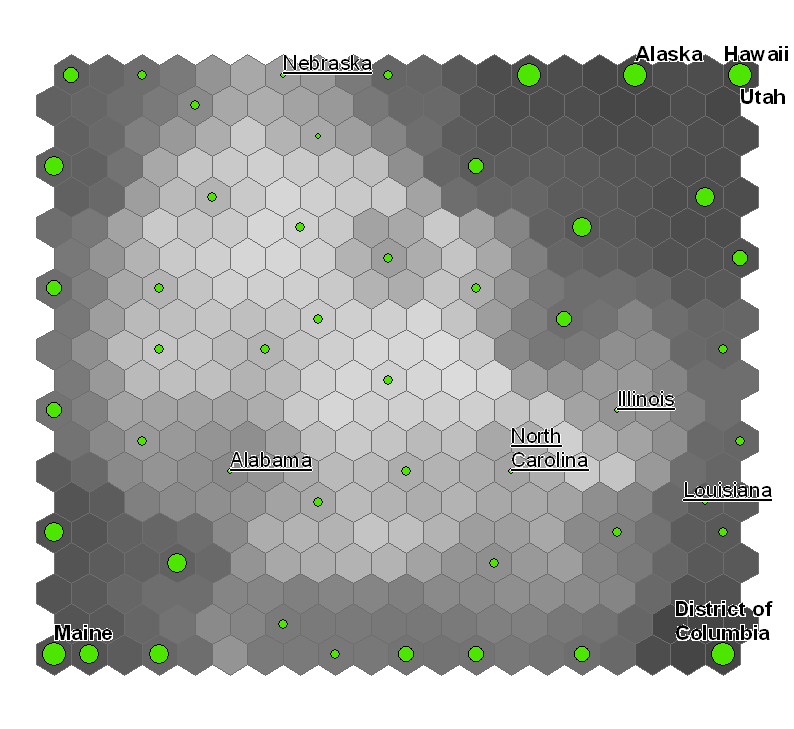
\includegraphics[width=0.70\linewidth]{states.png}
\end{center}
\end{figure}

One way to eliminate the edge effect is to wrap the lattice around a
three-dimensional object such as a sphere or torus, thereby removing the edge
entirely. The toroidal SOM was introduced by \cite{li1993}, however the torus
is not effective for visualization, as maps generated from a torus are not
very intuitive \cite{ito2000,wu2006}.  \cite{ritter99} describes the torus as
being topologically flat and suggests that a curved topology, such as that of
a sphere, may better reflect directional data.  A sphere also results in a
more intuitive map, since we are accustomed to looking at geographic maps
based on a sphere.  

\label{bg:sphere}
Ritter \cite{ritter99} first introduced the spherical SOM, and several enhancements have
since been suggested \cite{boudjemai2003,sangole03,Nishio:2006fk,wu2006}.  A
good comparison of these enhancements can be found in Wu and Takatsuka
 \cite{wu2006}.  All of
these methods derive their spherical structure through the tessellation of a
polyhedron as originally proposed by Ritter \cite{ritter99}.  Wu and Takatsuka \cite{wu2006} point
out the importance of a uniform distribution on the sphere, and that it is
preferable for all neurons to have an equal number of neighbors and to be
equally spaced.  They find generally that the tessellation method best satisfies
these conditions, and specifically that the icosahedron is the best starting
point \cite{wu2005}. Tessellation of the icosahedron results in a network of
neurons, each having exactly six neighbors, save the original twelve
which each have five neighbors.  This is very close to the ideal structure in
which every neuron would have exactly six neighbors.  \cite{wu2006} prefer
these this structure, because it has very low variances in both neuron spacing
and neighborhood size. 

Based solely on measures of neuron spacing, \cite{wu2005} dismissed the usefulness of a method
proposed by \cite{Rakhmanov94} for distributing points on a sphere.  Similarly
\cite{Nishio:2006fk} use these variance measures to support their helix
algorithm for distributing points on a sphere.  However,
these metrics can be misleading and comparison across topologies may not be
consistent.  The traditional rectangular and hexagonal topologies have no
variance in neuron spacing, and the generally preferred hexagonal structure
displays greater variance in neighborhood size than the rectangular structure.
The torus, by comparison, would have variance in neuron spacing, yet no
variance in neighborhood size.  The distance between two neurons is only
considered during the formation of the neural network.  At this stage the
spacing is significant as it plays a part in constructing the network's
topology by determining neuron adjacency.  However, using this measure to
evaluate potential topologies for use in SOM may be misleading.

As spherical (and other alternative) topologies become
increasingly more common it is necessary to investigate how the choice of
topology effects the SOM.  In this thesis the effect of irregularity within
topologies is studied as an attempt to investigate not only the edge effect,
but also to help facilitate the comparison of topologies.  It is important to
note that spherical topologies may not be appropriate for all applications.
Removing the edge may reduce the SOM's ability to converge.  As outliers are
forced to interact they introduce more competition among the neurons.  We
would also expect outliers to occupy more space in the final map as their
dissimilarity in attribute space should translate to more distant spatial
relationships in the trained SOM.  More research will be needed to help researches
determine the most appropriate topology for their data and research objectives.

In this paper we explore the general utility of certain irregular spherical
topologies beyond offering greater control over network size. We develop and
test new diagnostics to measure and visualize topology-induced errors in SOM.
More specifically we examine the



\Section{Methods}
We train SOMs using four different topologies:
\emph{rectangular, hexagonal, geodesic sphere} and \emph{spherical}.  The spherical
topology is based on a method, developed by \cite{Rakhmanov94}, for
distributing an arbitrary number of points on to the surface of a sphere.
Delaunay triangulation is then applied to these points, producing a
topological structure.  To yield meaningful results these SOMs must be trained
with comparable parameters.  The literature provides many rules of thumb for
training a SOM: each SOM is trained in two stages, the first of which uses a larger
initial learning rate and neighborhood search radius with a small number of
training steps; the second stage uses a lower initial learning rate and
neighborhood search radius, but extends the length of training.
\\
First Stage Parameters:
\begin{itemize}
  \item Initial neighborhood search radius of 50\%, which decreases during training. 
  \item Initial learning rate of 0.04 which decreases during training.
  \item 100,000 training steps.
\end{itemize}
Second Stage Parameters:
\begin{itemize}
  \item Initial neighborhood search radius of 33\%, which decreases during training. 
  \item Initial learning rate of 0.03 which decreases during training.
  \item 1,000,000 training steps.
\end{itemize}

As shown in Figure \ref{fig:nSize}, topologies differ in terms of achievable
network size.  For comparability, the network size of each SOM needs to be as
close as possible.  The achievable network size for the geodesic SOM is the
most limiting of the topologies we test. We chose the eighth frequency
geodesic sphere, which has 642 nodes, which is relatively close to the
644-node hexagonal and rectangular topologies achieved when the dimensions are
set to \(28x23\). Finally, the spherical topology was set to 642 nodes.

\begin{figure}[htb]
  \begin{center}
\caption{SOM Size and spherical topologies.}
\label{fig:nSize}
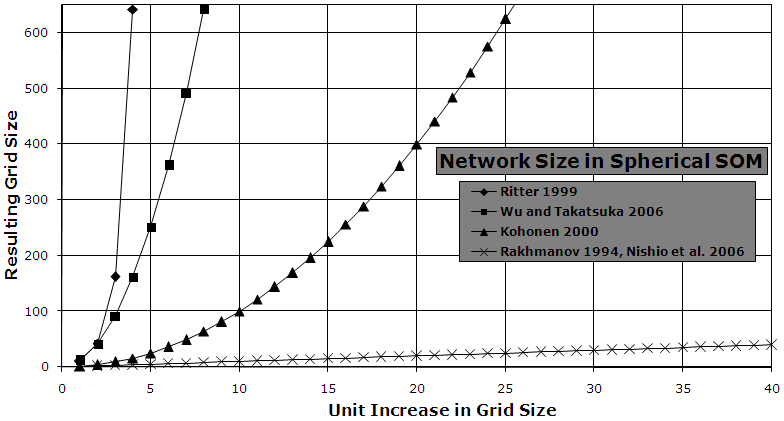
\includegraphics[width=0.70\linewidth]{networkSize.png}
\end{center}
\end{figure}

%------------------------------------------------------------------------- 

%------------------------------------------------------------------------- 
\SubSection{Language}

All manuscripts must be in English.

%------------------------------------------------------------------------- 
\SubSection{Printing your paper}

Print your properly formatted text on high-quality, $8.5 \times 11$-inch 
white printer paper. A4 paper is also acceptable, but please leave the 
extra 0.5 inch (1.27 cm) at the BOTTOM of the page.

%------------------------------------------------------------------------- 
\SubSection{Margins and page numbering}

All printed material, including text, illustrations, and charts, must be 
kept within a print area 6-7/8 inches (17.5 cm) wide by 8-7/8 inches 
(22.54 cm) high. Do not write or print anything outside the print area. 
Number your pages lightly, in pencil, on the upper right-hand corners of 
the BACKS of the pages (for example, 1/10, 2/10, or 1 of 10, 2 of 10, and 
so forth). Please do not write on the fronts of the pages, nor on the 
lower halves of the backs of the pages.


%------------------------------------------------------------------------ 
\SubSection{Formatting your paper}

All text must be in a two-column format. The total allowable width of 
the text area is 6-7/8 inches (17.5 cm) wide by 8-7/8 inches (22.54 cm) 
high. Columns are to be 3-1/4 inches (8.25 cm) wide, with a 5/16 inch 
(0.8 cm) space between them. The main title (on the first page) should 
begin 1.0 inch (2.54 cm) from the top edge of the page. The second and 
following pages should begin 1.0 inch (2.54 cm) from the top edge. On 
all pages, the bottom margin should be 1-1/8 inches (2.86 cm) from the 
bottom edge of the page for $8.5 \times 11$-inch paper; for A4 paper, 
approximately 1-5/8 inches (4.13 cm) from the bottom edge of the page.

%------------------------------------------------------------------------- 
\SubSection{Type-style and fonts}

Wherever Times is specified, Times Roman may also be used. If neither is 
available on your word processor, please use the font closest in 
appearance to Times that you have access to.

MAIN TITLE. Center the title 1-3/8 inches (3.49 cm) from the top edge of 
the first page. The title should be in Times 14-point, boldface type. 
Capitalize the first letter of nouns, pronouns, verbs, adjectives, and 
adverbs; do not capitalize articles, coordinate conjunctions, or 
prepositions (unless the title begins with such a word). Leave two blank 
lines after the title.

AUTHOR NAME(s) and AFFILIATION(s) are to be centered beneath the title 
and printed in Times 12-point, non-boldface type. This information is to 
be followed by two blank lines.

The ABSTRACT and MAIN TEXT are to be in a two-column format. 

MAIN TEXT. Type main text in 10-point Times, single-spaced. Do NOT use 
double-spacing. All paragraphs should be indented 1 pica (approx. 1/6 
inch or 0.422 cm). Make sure your text is fully justified---that is, 
flush left and flush right. Please do not place any additional blank 
lines between paragraphs. Figure and table captions should be 10-point 
Helvetica boldface type as in
\begin{figure}[h]
   \caption{Example of caption.}
\end{figure}

\noindent Long captions should be set as in 
\begin{figure}[h] 
   \caption{Example of long caption requiring more than one line. It is 
     not typed centered but aligned on both sides and indented with an 
     additional margin on both sides of 1~pica.}
\end{figure}

\noindent Callouts should be 9-point Helvetica, non-boldface type. 
Initially capitalize only the first word of section titles and first-, 
second-, and third-order headings.

FIRST-ORDER HEADINGS. (For example, {\large \bf 1. Introduction}) 
should be Times 12-point boldface, initially capitalized, flush left, 
with one blank line before, and one blank line after.

SECOND-ORDER HEADINGS. (For example, {\elvbf 1.1. Database elements}) 
should be Times 11-point boldface, initially capitalized, flush left, 
with one blank line before, and one after. If you require a third-order 
heading (we discourage it), use 10-point Times, boldface, initially 
capitalized, flush left, preceded by one blank line, followed by a period 
and your text on the same line.

%------------------------------------------------------------------------- 
\SubSection{Footnotes}

Please use footnotes sparingly%
\footnote
   {%
     Or, better still, try to avoid footnotes altogether.  To help your 
     readers, avoid using footnotes altogether and include necessary 
     peripheral observations in the text (within parentheses, if you 
     prefer, as in this sentence).
   }
and place them at the bottom of the column on the page on which they are 
referenced. Use Times 8-point type, single-spaced.


%------------------------------------------------------------------------- 
\SubSection{References}

List and number all bibliographical references in 9-point Times, 
single-spaced, at the end of your paper. When referenced in the text, 
enclose the citation number in square brackets, for example~\cite{ex1}. 
Where appropriate, include the name(s) of editors of referenced books.

%------------------------------------------------------------------------- 
\SubSection{Illustrations, graphs, and photographs}

All graphics should be centered. Your artwork must be in place in the 
article (preferably printed as part of the text rather than pasted up). 
If you are using photographs and are able to have halftones made at a 
print shop, use a 100- or 110-line screen. If you must use plain photos, 
they must be pasted onto your manuscript. Use rubber cement to affix the 
images in place. Black and white, clear, glossy-finish photos are 
preferable to color. Supply the best quality photographs and 
illustrations possible. Penciled lines and very fine lines do not 
reproduce well. Remember, the quality of the book cannot be better than 
the originals provided. Do NOT use tape on your pages!

%------------------------------------------------------------------------- 
\SubSection{Color}

The use of color on interior pages (that is, pages other
than the cover) is prohibitively expensive. We publish interior pages in 
color only when it is specifically requested and budgeted for by the 
conference organizers. DO NOT SUBMIT COLOR IMAGES IN YOUR 
PAPERS UNLESS SPECIFICALLY INSTRUCTED TO DO SO.

%------------------------------------------------------------------------- 
\SubSection{Symbols}

If your word processor or typewriter cannot produce Greek letters, 
mathematical symbols, or other graphical elements, please use 
pressure-sensitive (self-adhesive) rub-on symbols or letters (available 
in most stationery stores, art stores, or graphics shops).

%------------------------------------------------------------------------ 
\SubSection{Copyright forms}

You must include your signed IEEE copyright release form when you submit 
your finished paper. We MUST have this form before your paper can be 
published in the proceedings.

%------------------------------------------------------------------------- 
\SubSection{Conclusions}

Please direct any questions to the production editor in charge of these 
proceedings at the IEEE Computer Society Press: Phone (714) 821-8380, or 
Fax (714) 761-1784.

%------------------------------------------------------------------------- 
\nocite{ex1,ex2}
\bibliographystyle{latex8}
\bibliography{../proposal/som}

\end{document}

